% Note that the a4paper option is mainly intended so that authors in
% countries using A4 can easily print to A4 and see how their papers will
% look in print - the typesetting of the document will not typically be
% affected with changes in paper size (but the bottom and side margins will).
% Use the testflow package mentioned above to verify correct handling of
% both paper sizes by the user's LaTeX system.
%
% Also note that the "draftcls" or "draftclsnofoot", not "draft", option
% should be used if it is desired that the figures are to be displayed in
% draft mode.
%
\documentclass[conference]{IEEEtran}
% Add the compsoc option for Computer Society conferences.
%
% If IEEEtran.cls has not been installed into the LaTeX system files,
% manually specify the path to it like:
% \documentclass[conference]{../sty/IEEEtran}





% Some very useful LaTeX packages include:
% (uncomment the ones you want to load)


% *** MISC UTILITY PACKAGES ***
%
%\usepackage{ifpdf}
% Heiko Oberdiek's ifpdf.sty is very useful if you need conditional
% compilation based on whether the output is pdf or dvi.
% usage:
% \ifpdf
%   % pdf code
% \else
%   % dvi code
% \fi
% The latest version of ifpdf.sty can be obtained from:
% http://www.ctan.org/tex-archive/macros/latex/contrib/oberdiek/
% Also, note that IEEEtran.cls V1.7 and later provides a builtin
% \ifCLASSINFOpdf conditional that works the same way.
% When switching from latex to pdflatex and vice-versa, the compiler may
% have to be run twice to clear warning/error messages.






% *** CITATION PACKAGES ***
%
%\usepackage{cite}
% cite.sty was written by Donald Arseneau
% V1.6 and later of IEEEtran pre-defines the format of the cite.sty package
% \cite{} output to follow that of IEEE. Loading the cite package will
% result in citation numbers being automatically sorted and properly
% "compressed/ranged". e.g., [1], [9], [2], [7], [5], [6] without using
% cite.sty will become [1], [2], [5]--[7], [9] using cite.sty. cite.sty's
% \cite will automatically add leading space, if needed. Use cite.sty's
% noadjust option (cite.sty V3.8 and later) if you want to turn this off.
% cite.sty is already installed on most LaTeX systems. Be sure and use
% version 4.0 (2003-05-27) and later if using hyperref.sty. cite.sty does
% not currently provide for hyperlinked citations.
% The latest version can be obtained at:
% http://www.ctan.org/tex-archive/macros/latex/contrib/cite/
% The documentation is contained in the cite.sty file itself.






% *** GRAPHICS RELATED PACKAGES ***
%
\ifCLASSINFOpdf
  \usepackage[pdftex]{graphicx}
  % declare the path(s) where your graphic files are
  \graphicspath{{../Output/}{/}}
  % and their extensions so you won't have to specify these with
  % every instance of \includegraphics
  \DeclareGraphicsExtensions{.pdf,.jpeg,.jpg,.png}
\else
  % or other class option (dvipsone, dvipdf, if not using dvips). graphicx
  % will default to the driver specified in the system graphics.cfg if no
  % driver is specified.
  % \usepackage[dvips]{graphicx}
  % declare the path(s) where your graphic files are
  % \graphicspath{{../eps/}}
  % and their extensions so you won't have to specify these with
  % every instance of \includegraphics
  % \DeclareGraphicsExtensions{.eps}
\fi
% graphicx was written by David Carlisle and Sebastian Rahtz. It is
% required if you want graphics, photos, etc. graphicx.sty is already
% installed on most LaTeX systems. The latest version and documentation can
% be obtained at: 
% http://www.ctan.org/tex-archive/macros/latex/required/graphics/
% Another good source of documentation is "Using Imported Graphics in
% LaTeX2e" by Keith Reckdahl which can be found as epslatex.ps or
% epslatex.pdf at: http://www.ctan.org/tex-archive/info/
%
% latex, and pdflatex in dvi mode, support graphics in encapsulated
% postscript (.eps) format. pdflatex in pdf mode supports graphics
% in .pdf, .jpeg, .png and .mps (metapost) formats. Users should ensure
% that all non-photo figures use a vector format (.eps, .pdf, .mps) and
% not a bitmapped formats (.jpeg, .png). IEEE frowns on bitmapped formats
% which can result in "jaggedy"/blurry rendering of lines and letters as
% well as large increases in file sizes.
%
% You can find documentation about the pdfTeX application at:
% http://www.tug.org/applications/pdftex





% *** MATH PACKAGES ***
%
\usepackage[cmex10]{amsmath}
% A popular package from the American Mathematical Society that provides
% many useful and powerful commands for dealing with mathematics. If using
% it, be sure to load this package with the cmex10 option to ensure that
% only type 1 fonts will utilized at all point sizes. Without this option,
% it is possible that some math symbols, particularly those within
% footnotes, will be rendered in bitmap form which will result in a
% document that can not be IEEE Xplore compliant!
%
% Also, note that the amsmath package sets \interdisplaylinepenalty to 10000
% thus preventing page breaks from occurring within multiline equations. Use:
%\interdisplaylinepenalty=2500
% after loading amsmath to restore such page breaks as IEEEtran.cls normally
% does. amsmath.sty is already installed on most LaTeX systems. The latest
% version and documentation can be obtained at:
% http://www.ctan.org/tex-archive/macros/latex/required/amslatex/math/





% *** SPECIALIZED LIST PACKAGES ***
%
%\usepackage{algorithmic}
% algorithmic.sty was written by Peter Williams and Rogerio Brito.
% This package provides an algorithmic environment fo describing algorithms.
% You can use the algorithmic environment in-text or within a figure
% environment to provide for a floating algorithm. Do NOT use the algorithm
% floating environment provided by algorithm.sty (by the same authors) or
% algorithm2e.sty (by Christophe Fiorio) as IEEE does not use dedicated
% algorithm float types and packages that provide these will not provide
% correct IEEE style captions. The latest version and documentation of
% algorithmic.sty can be obtained at:
% http://www.ctan.org/tex-archive/macros/latex/contrib/algorithms/
% There is also a support site at:
% http://algorithms.berlios.de/index.html
% Also of interest may be the (relatively newer and more customizable)
% algorithmicx.sty package by Szasz Janos:
% http://www.ctan.org/tex-archive/macros/latex/contrib/algorithmicx/




% *** ALIGNMENT PACKAGES ***
%
\usepackage{array}
% Frank Mittelbach's and David Carlisle's array.sty patches and improves
% the standard LaTeX2e array and tabular environments to provide better
% appearance and additional user controls. As the default LaTeX2e table
% generation code is lacking to the point of almost being broken with
% respect to the quality of the end results, all users are strongly
% advised to use an enhanced (at the very least that provided by array.sty)
% set of table tools. array.sty is already installed on most systems. The
% latest version and documentation can be obtained at:
% http://www.ctan.org/tex-archive/macros/latex/required/tools/


%\usepackage{mdwmath}
%\usepackage{mdwtab}
% Also highly recommended is Mark Wooding's extremely powerful MDW tools,
% especially mdwmath.sty and mdwtab.sty which are used to format equations
% and tables, respectively. The MDWtools set is already installed on most
% LaTeX systems. The lastest version and documentation is available at:
% http://www.ctan.org/tex-archive/macros/latex/contrib/mdwtools/


% IEEEtran contains the IEEEeqnarray family of commands that can be used to
% generate multiline equations as well as matrices, tables, etc., of high
% quality.


%\usepackage{eqparbox}
% Also of notable interest is Scott Pakin's eqparbox package for creating
% (automatically sized) equal width boxes - aka "natural width parboxes".
% Available at:
% http://www.ctan.org/tex-archive/macros/latex/contrib/eqparbox/





% *** SUBFIGURE PACKAGES ***
\usepackage[tight,footnotesize]{subfigure}
% subfigure.sty was written by Steven Douglas Cochran. This package makes it
% easy to put subfigures in your figures. e.g., "Figure 1a and 1b". For IEEE
% work, it is a good idea to load it with the tight package option to reduce
% the amount of white space around the subfigures. subfigure.sty is already
% installed on most LaTeX systems. The latest version and documentation can
% be obtained at:
% http://www.ctan.org/tex-archive/obsolete/macros/latex/contrib/subfigure/
% subfigure.sty has been superceeded by subfig.sty.



%\usepackage[caption=false]{caption}
%\usepackage[font=footnotesize]{subfig}
% subfig.sty, also written by Steven Douglas Cochran, is the modern
% replacement for subfigure.sty. However, subfig.sty requires and
% automatically loads Axel Sommerfeldt's caption.sty which will override
% IEEEtran.cls handling of captions and this will result in nonIEEE style
% figure/table captions. To prevent this problem, be sure and preload
% caption.sty with its "caption=false" package option. This is will preserve
% IEEEtran.cls handing of captions. Version 1.3 (2005/06/28) and later 
% (recommended due to many improvements over 1.2) of subfig.sty supports
% the caption=false option directly:
%\usepackage[caption=false,font=footnotesize]{subfig}
%
% The latest version and documentation can be obtained at:
% http://www.ctan.org/tex-archive/macros/latex/contrib/subfig/
% The latest version and documentation of caption.sty can be obtained at:
% http://www.ctan.org/tex-archive/macros/latex/contrib/caption/




% *** FLOAT PACKAGES ***
%
%\usepackage{fixltx2e}
% fixltx2e, the successor to the earlier fix2col.sty, was written by
% Frank Mittelbach and David Carlisle. This package corrects a few problems
% in the LaTeX2e kernel, the most notable of which is that in current
% LaTeX2e releases, the ordering of single and double column floats is not
% guaranteed to be preserved. Thus, an unpatched LaTeX2e can allow a
% single column figure to be placed prior to an earlier double column
% figure. The latest version and documentation can be found at:
% http://www.ctan.org/tex-archive/macros/latex/base/



%\usepackage{stfloats}
% stfloats.sty was written by Sigitas Tolusis. This package gives LaTeX2e
% the ability to do double column floats at the bottom of the page as well
% as the top. (e.g., "\begin{figure*}[!b]" is not normally possible in
% LaTeX2e). It also provides a command:
%\fnbelowfloat
% to enable the placement of footnotes below bottom floats (the standard
% LaTeX2e kernel puts them above bottom floats). This is an invasive package
% which rewrites many portions of the LaTeX2e float routines. It may not work
% with other packages that modify the LaTeX2e float routines. The latest
% version and documentation can be obtained at:
% http://www.ctan.org/tex-archive/macros/latex/contrib/sttools/
% Documentation is contained in the stfloats.sty comments as well as in the
% presfull.pdf file. Do not use the stfloats baselinefloat ability as IEEE
% does not allow \baselineskip to stretch. Authors submitting work to the
% IEEE should note that IEEE rarely uses double column equations and
% that authors should try to avoid such use. Do not be tempted to use the
% cuted.sty or midfloat.sty packages (also by Sigitas Tolusis) as IEEE does
% not format its papers in such ways.





% *** PDF, URL AND HYPERLINK PACKAGES ***
%
\usepackage{url}
% url.sty was written by Donald Arseneau. It provides better support for
% handling and breaking URLs. url.sty is already installed on most LaTeX
% systems. The latest version can be obtained at:
% http://www.ctan.org/tex-archive/macros/latex/contrib/misc/
% Read the url.sty source comments for usage information. Basically,
% \url{my_url_here}.





% *** Do not adjust lengths that control margins, column widths, etc. ***
% *** Do not use packages that alter fonts (such as pslatex).         ***
% There should be no need to do such things with IEEEtran.cls V1.6 and later.
% (Unless specifically asked to do so by the journal or conference you plan
% to submit to, of course. )


% correct bad hyphenation here
\hyphenation{op-tical net-works semi-conduc-tor}


\begin{document}
%
% paper title
% can use linebreaks \\ within to get better formatting as desired
\title{Line extraction via profile analysis 
with prior foreground segmentation using cues.}

% author names and affiliations
% use a multiple column layout for up to three different
% affiliations
\author{\IEEEauthorblockN{Michael Single}
\IEEEauthorblockA{University of Berne\\
08-917-445}
\and
\IEEEauthorblockN{Stefan Moser}
\IEEEauthorblockA{University of Berne\\
09-277-013}
}

% make the title area
\maketitle

\section{Motivation}
Although there exist many sophisticated image processing algorithms, 
extracting text lines from arbitrary formatted text documents is nowadays still an not generally solved issue. 
There are many problems that may arise when addressing this problem. 
The written text can either be hand-or/and machine written, 
the text can exhibit an unknown formatting 
(especially, when dealing with human handwritings) 
or the document itself might suffer from different types of artifacts or deformations. 

\section{Problem Statement}
In this work we describe an algorithm that allows us to extract text lines from different types of documents. 
In practise we are dealing with both, 
hand and machine-written, texts. 
The extracted text lines may then used for further analysis such as character recognition or layout analysis.

\section{Algorithm}
First, we extract the scripture\footnote{subsequently called foreground} 
using cues, then we do profile analysis on it and finally construct a 
convex hull around every individual line using the results of the two previous steps. 
In the following we describe each individual step in further detail.

\subsection{Foreground/Background segmentation}
Given a certain document that exhibits some human and machine writings,
 our first task is to extract the included text from its background. 
 For the purpose of extracting the fore-and background of an image, 
 we rely on a supervised binary image segmentation algorithm. 
 This means, given some user specified cues that are labelling some pixels in the image $\footnote{labelling a pixel means marking it whether it belongs to the image's fore-or background}$, 
 we want to find an optimal binary image s.t. each pixel is assigned to a label and matches the cues. 
 This problem statement can be addressed by formulating the problem as an energy minimization problem. 

This energy E depends on two terms: a \emph{data}-and a \emph{smoothness}-term. 
The smoothness term describes the desired relationship between neighboring pixels whereas the data term is encoding the probability for certain output pixel value$\footnote{i.e. probability, that a pixel belongs to a certain label}$. 
The described optimization problem can be numerically solved by constructing an appropriate weighted flow graph and then computing its minimum cut. 
This cut value corresponds to the minimal energy. 
This flow graph is constructed as the following procedure describes:
\begin{itemize}
	\item For each pixel in the given image, we add a node to the graph. Two additional nodes are added to the graph, one for each binary label called F and B.
	\item We represent the smoothness term by adding edges between each pair of neighboring pixel-nodes in the graph. The the data term is represented by connecting each pixel-node with both label-nodes. 
	\item The edge-weights are determined by the data and smoothness term values from a corresponding pixel.
\end{itemize}

Using the described weighted flow graph, we can find an optimal labelling by solving for its minimum cut. A cut removes edges to disconnect the label F from the label Node B (i.e. there is no path from F to B). Thus, the min. cut is minimized sum of cut edge weights. The minimum cut can be determined by the ford \emph{Fulkerson's algorithm}. 

In summary, our segmentation algorithm performs the following steps:
\begin{enumerate}
	\item Our implementation expects a user to first brush some strokes on the image that indicate whether a particular pixel belongs to the image’s fore-or background.
	\item Model the probability for each pixel to belong to foreground or background. In order to do so, collect histograms of pixels colors covered by foreground and background strokes. The histogram$\footnote{Instead of using 3d color histograms we make use of gaussian mixture models to estimate the color distibution.}$ represents probability distribution of color values and models a pixel’s data term. the data term for a pixel is high valued if the corresponding probability is close to zero.
	\item Label boundaries should coincide with edges, should avoid boundaries in smooth areas. If labels are the same then term is zero, otherwise cost is high if pixel values are similar (use an exp. function). visit neighborhood of a pixel and compute this term by traversing its neighbors.
	\item Construct the flow graph and solve for its minimum cut by using the \emph{GCMEX}\cite{Fulkerson2009} library.
	\item The minimum cut value corresponds to the minimized energy function E.
\end{enumerate}

\subsection{Line retrieval}
Using the foreground retrieved in the last analysis, we now apply profile analysis  \cite{ciardiello1988experimental}, which is a well proven technique in the domain of document analysis:
For every row of the image, we count the number of black pixels, as displayed to the right of Figure \ref{fig:profile_analysis}. 
After a normalization step, we then choose a threshold\footnote{By analyzing the histogram of the profile} to map the profile to binary rows (See Figure \ref{fig:Results:line_image}).

While this is usually also done along the columns, 
this only lead to complications without any improvements in our image set and was left out for this reason.
\begin{figure}[ht!]%
\centering
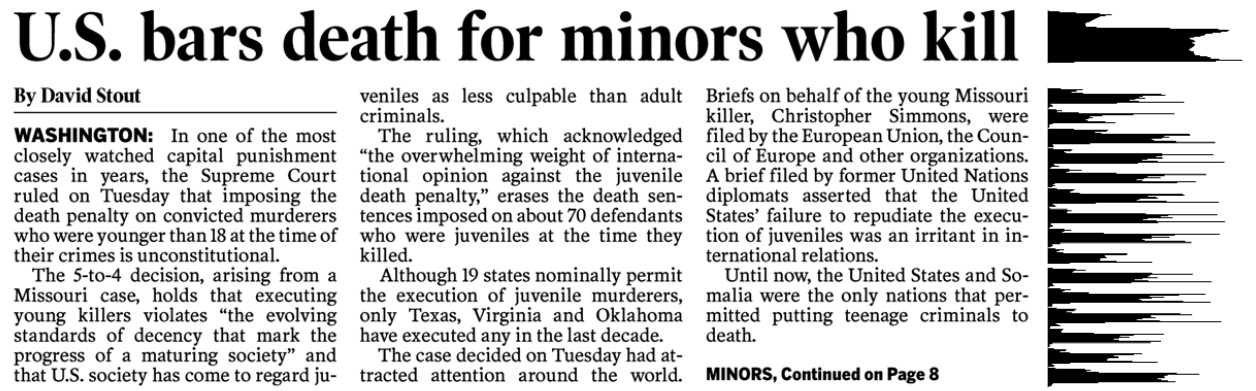
\includegraphics[width=0.45\textwidth]{profile_analysis}
\caption{Visualisation of the results of profile analysis along the rows. Image taken from lecture.}
\label{fig:profile_analysis}
\end{figure}
Results from this procedure are however not very robust for handwriting.
Lots of characters overflow from their lines and lead to false positives as well
as false negatives in between lines. 
But these errors all share the trait of being very small 
- usually around 5 pixels at maximum. 
So we decided to sanitize the results by doing a run elimination for both small runs of zeros 
(reject tiny gaps in lines) as well as ones 
(reject lines that are too small, too far from other lines).
This lead to much more satisfying results.

\subsection{Constructing convex hull}
In a last step, we combine the results from the two previous steps
to construct a rather tight convex hull around the lines found.
For this purpose we iterate over every line retrieved in the profile
analysis and check 
which connected components of the foreground are overlapping with it.
If there is an overlap of more than 5 pixels, 
we assign the component to this line and mark it to prevent assigning
it again to another line.

In order for getting rid of small outliers, 
we check if the sum of connected components in the pixels assigned to a line is below a certain threshold (100 pixels in our case). 
If it is, we reject the line at this point.

Once we gathered all connected components belonging to the line, 
we iterate over the rows of unified connected components and find its
extent. 
For every row this gives us two points 
(to the far left and the far right) that we add to our convex hull.
\section{Results}
Using the algorithm described above we could produce decent results for a data set with mixed hand- and machine-written scripture. 
The final result including the intermediary outputs can be seen in Figure \ref{fig:Results}.
\begin{figure}[ht!]%
\centering
\subfigure[Initial image]{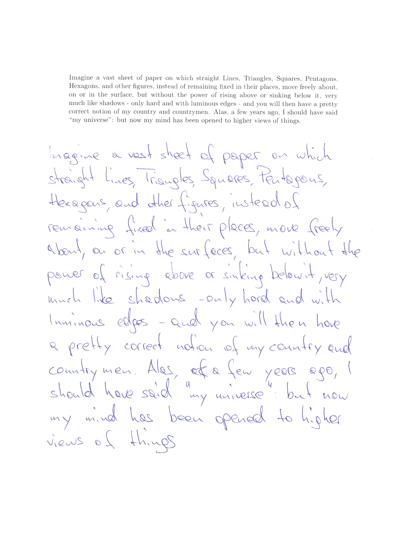
\includegraphics[width=0.23\textwidth]{0012-1_rescaled}}
\subfigure[Foreground]{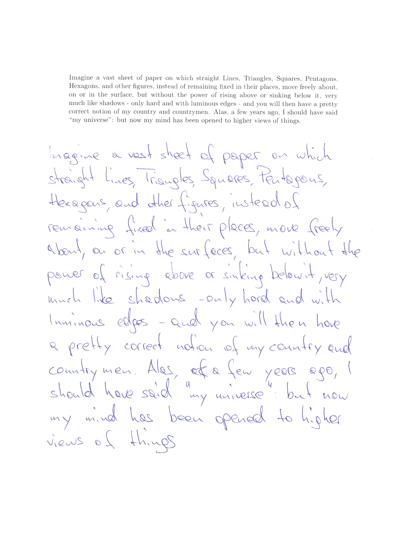
\includegraphics[width=0.23\textwidth]{0012-1_rescaled}}\\
\subfigure[Lines from profile analysis]{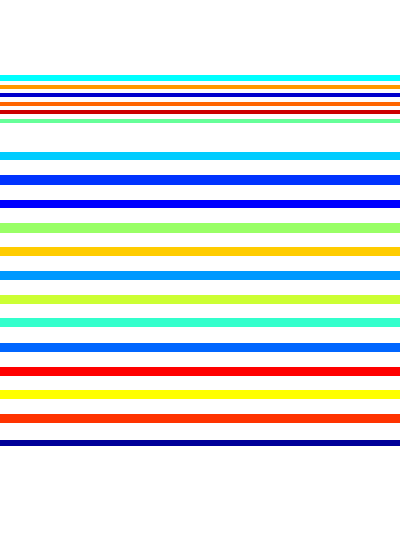
\includegraphics[width=0.23\textwidth]{0012-1_labeled_rows}
\label{fig:Results:line_image}}
\subfigure[Reconstructed convex hulls]{
\includegraphics[width=0.23\textwidth]{0012-1_convex_hulls}}
\caption{Results of our line extraction pipeline.}
\label{fig:Results}
\end{figure}

\section{Conclusion}
While this algorithm works well if the lines are well aligned\footnote{i. e. parallel to the x-axis of the image}, 
it completely fails if this condition is not met.
Due to time restriction, 
we were not able to add a preprocessing component that justifies the lines.

Additionally, instead of constructing convex hulls around the connected components
retrieved, we could construct polygons that could possibly add a tighter boundary.

% An example of a floating figure using the graphicx package.
% Note that \label must occur AFTER (or within) \caption.
% For figures, \caption should occur after the \includegraphics.
% Note that IEEEtran v1.7 and later has special internal code that
% is designed to preserve the operation of \label within \caption
% even when the captionsoff option is in effect. However, because
% of issues like this, it may be the safest practice to put all your
% \label just after \caption rather than within \caption{}.
%
% Reminder: the "draftcls" or "draftclsnofoot", not "draft", class
% option should be used if it is desired that the figures are to be
% displayed while in draft mode.
%
%\begin{figure}[!t]
%\centering
%\includegraphics[width=2.5in]{myfigure}
% where an .eps filename suffix will be assumed under latex, 
% and a .pdf suffix will be assumed for pdflatex; or what has been declared
% via \DeclareGraphicsExtensions.
%\caption{Simulation Results}
%\label{fig_sim}
%\end{figure}

% Note that IEEE typically puts floats only at the top, even when this
% results in a large percentage of a column being occupied by floats.


% An example of a double column floating figure using two subfigures.
% (The subfig.sty package must be loaded for this to work.)
% The subfigure \label commands are set within each subfloat command, the
% \label for the overall figure must come after \caption.
% \hfil must be used as a separator to get equal spacing.
% The subfigure.sty package works much the same way, except \subfigure is
% used instead of \subfloat.
%
%\begin{figure*}[!t]
%\centerline{\subfloat[Case I]\includegraphics[width=2.5in]{subfigcase1}%
%\label{fig_first_case}}
%\hfil
%\subfloat[Case II]{\includegraphics[width=2.5in]{subfigcase2}%
%\label{fig_second_case}}}
%\caption{Simulation results}
%\label{fig_sim}
%\end{figure*}
%
% Note that often IEEE papers with subfigures do not employ subfigure
% captions (using the optional argument to \subfloat), but instead will
% reference/describe all of them (a), (b), etc., within the main caption.


% An example of a floating table. Note that, for IEEE style tables, the 
% \caption command should come BEFORE the table. Table text will default to
% \footnotesize as IEEE normally uses this smaller font for tables.
% The \label must come after \caption as always.
%
%\begin{table}[!t]
%% increase table row spacing, adjust to taste
%\renewcommand{\arraystretch}{1.3}
% if using array.sty, it might be a good idea to tweak the value of
% \extrarowheight as needed to properly center the text within the cells
%\caption{An Example of a Table}
%\label{table_example}
%\centering
%% Some packages, such as MDW tools, offer better commands for making tables
%% than the plain LaTeX2e tabular which is used here.
%\begin{tabular}{|c||c|}
%\hline
%One & Two\\
%\hline
%Three & Four\\
%\hline
%\end{tabular}
%\end{table}


% Note that IEEE does not put floats in the very first column - or typically
% anywhere on the first page for that matter. Also, in-text middle ("here")
% positioning is not used. Most IEEE journals/conferences use top floats
% exclusively. Note that, LaTeX2e, unlike IEEE journals/conferences, places
% footnotes above bottom floats. This can be corrected via the \fnbelowfloat
% command of the stfloats package.


% trigger a \newpage just before the given reference
% number - used to balance the columns on the last page
% adjust value as needed - may need to be readjusted if
% the document is modified later
%\IEEEtriggeratref{8}
% The "triggered" command can be changed if desired:
%\IEEEtriggercmd{\enlargethispage{-5in}}

\bibliographystyle{IEEEtran}
\bibliography{IEEEabrv,report}
\end{document}

